\subsubsection{Regresión lineal}


En realidad, la arquitectura de la red en la figura \ref{fig:xorgatenetwork} usa una neurona que tiene como objetivo simular una puerta lógica OR ($L_{1,1}$) y otra neurona una puerta lógica AND ($L_{1,2}$). Viendo la lógica de una puerta XOR:
\begin{eqnarray}
    A \oplus B = (A \land \neg B) \lor (\neg A \land B) = (A \lor B) \land (\neg A \lor \neg B)
\end{eqnarray}

Tiene sentido que se usen las puertas OR y AND en la red. Se puede ver gráficamente el funcionamiento de cada neurona en la siguiente imagen:
\begin{figure}[H]
    \centering
    
\includegraphics[width=15cm]{images/state-of-art/regression/xor.png}
    \caption{Puertas lógicas OR($L_{1,1}$), AND($L_{1,2}$) y XOR($L_{2,1}$)}
    \label{fig:orandxorgraph}
\end{figure}

Cada una de estas neuronas está realizando una tarea de clasificación, simplemente comprueba si los datos de entrada se encuentran en un lado o en otro de la recta. Esto es así porque se ha definido el perceptrón de tal forma que solo pueda devolver $0$ o $1$. Pero eliminando ese paso de clasificación que se ha definido en la ecuación \ref{eqn:perceptron}, se obtendría una regresión lineal tal que:
\begin{eqnarray}
  y = w \cdot x + b
      \label{eqn:neuronsimple}
\end{eqnarray}

Una regresión lineal es el otro tipo de tarea que una neurona puede resolver. Esta es una de las principales diferencias entre las neuronas modernas y los perceptrones. Los perceptrones solo están programados para realizar una tarea de clasificación, pero las neuronas se pueden programar para otro tipo de casos. Aunque como se explicará posteriormente, un perceptrón es un tipo de neurona con una función de activación escalonada (ver apartado \ref{activationfunction}).
\newline

\begin{figure}[H]
    \centering
    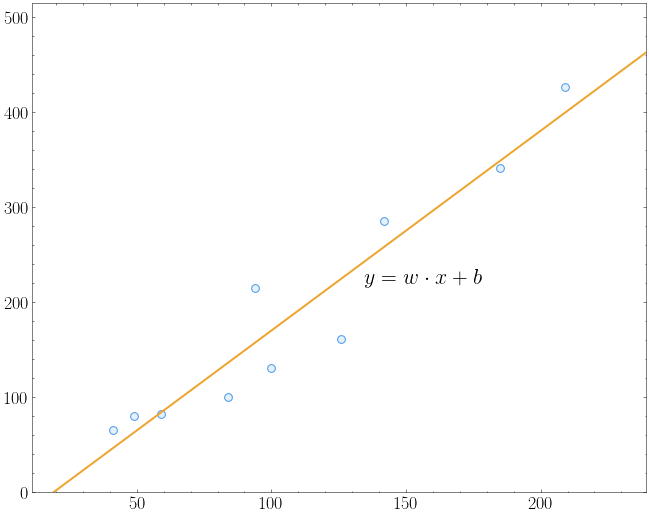
\includegraphics[width=9cm]{images/state-of-art/regression/regression.png}
    \caption{Ejemplo de regresión lineal en un espacio bidimensional}
    \label{fig:regression}
\end{figure}

Una regresión lineal es un método que estudia la relación existente entre varias variables y de ese modo genera un modelo que puede ser usado para estimar otros valores. Matemáticamente, en un espacio multidimensional $n$, una regresión se define de la siguiente manera:
\begin{eqnarray}
  y = w_0 + w_1x_1 + w_2x_2 + ... + w_nx_n
  \label{linealregression}
\end{eqnarray}


En esta ecuación hay un término independiente $w_0$, y por cada dimensión, habrá un valor $w$ y un valor $x$ asociado a ella. Geométricamente, en un espacio de dos dimensiones, $z$ será una recta, un plano si si son tres dimensiones y un hyperplano para mayores de tres dimensiones, que gráficamente no se puede representar. De hecho, se puede observar que la ecuación \ref{eqn:neuronsimple} es en realidad la función de una recta, siendo $b$ el término independiente. 
\newline

A partir de este punto se usará $z$ para referirse a la regresión lineal que es calculada en una neurona:
\begin{equation}
  z \equiv y = w \cdot x + b
  \label{eqn:z_equation_init}
\end{equation}

% Un ejemplo visual para mostrar la regresión lineal podría ser el siguiente. Usando $b=0.5$, la recta que quedaría sería:

% TODO AÑadir imagen con colores azul y rojo

% Añadir nota: La zona en azul sería la zona, donde $y=0$ y la zona en verde donde $y=1$. 
% \newline



